\documentclass[aspectratio=169,9pt]{beamer}
\usetheme[progressbar=frametitle,numbering=fraction]{metropolis}
\usepackage[utf8]{inputenc}
\usepackage[T1]{fontenc}
\usepackage{amsmath,amssymb}
\usepackage{graphicx}
\usepackage{booktabs}
\usepackage{tabularx}
\usepackage{siunitx}
\usepackage{tikz}
\usetikzlibrary{arrows.meta,decorations.pathmorphing,calc,patterns}
\sisetup{detect-all,range-phrase=--,range-units=single}

\definecolor{cBlue}{HTML}{2A6FBB}
\definecolor{cRed}{HTML}{D62839}
\definecolor{cDRed}{HTML}{7A0010}
\definecolor{cGreen}{HTML}{2A9D55}
\definecolor{cTeal}{HTML}{17A2B8}
\definecolor{cOrange}{HTML}{B5651D}
\definecolor{cPurple}{HTML}{8E44AD}
\newcommand{\tagM}{\textcolor{cGreen}{\textbf{[measured]}}}
\newcommand{\tagC}{\textcolor{cOrange}{\textbf{[computed]}}}
\newcommand{\tagD}{\textcolor{cPurple}{\textbf{[detected]}}}
\newcommand{\tagMo}{\textcolor{cRed}{\textbf{[model]}}}
\setbeamerfont{footnote}{size=\tiny}

\title{Adhesion properties from AFM retract curves}
\subtitle{What each quantity means, where it sits on the force curve, and how it is obtained}
\date{Worked example: data\_213626 (Ciona embryo, colloidal probe)}
\author{}

\begin{document}

\maketitle

% ---------------------------------------------------------------------------
\begin{frame}{Contents}
\begin{enumerate}
\item The data: which part of the force curve is used, units, sign convention
\item \textbf{Overview}: all adhesion properties on one force curve
\item Tip position instead of stage position
\item Read directly from the curve: zero-force point $s_0$, adhesion force $F_\text{adh}$, pull-off distance
\item Noise threshold $\to$ detachment length and ``detached'' flag
\item Work of adhesion $W$ (integral)
\item Rupture events (step detection)
\item Membrane tether plateaus
\item JKR work of adhesion per area $w$ (contact model)
\item Typical values, example maps, all parameters, limitations
\end{enumerate}
\end{frame}

% ---------------------------------------------------------------------------
\section{The data}

\begin{frame}{One force curve: approach and retract}
\centering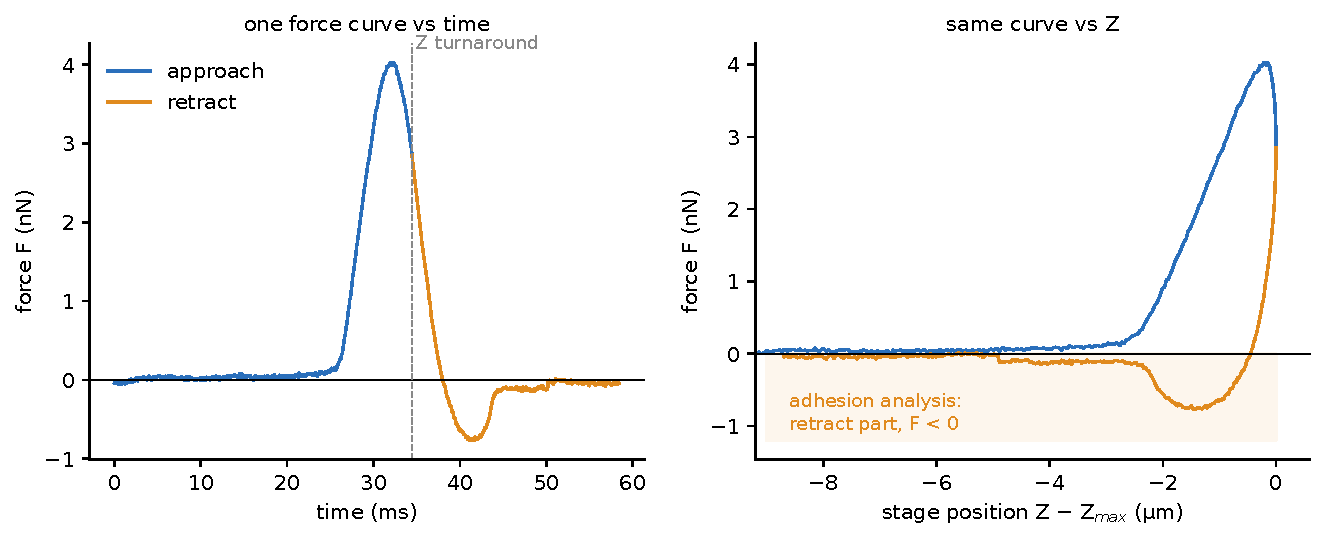
\includegraphics[height=0.52\textheight]{fig/full_curve.pdf}
\begin{itemize}\small
\item Approach (blue): probe pushed into the cell until the trigger force; retract (orange): probe pulled back.
\item \textbf{All adhesion properties come from the retract part only}: every point after the \textbf{Z turnaround} (maximum of the stage position), \num{\approx 330} points, \num{\approx 8.7}\,\si{\micro\metre} of travel, \num{\approx 24}\,\si{\milli\second}.
\item Adhesion = the part of the retract curve where the force is \textbf{negative} (the sample pulls on the probe).
\end{itemize}
\end{frame}

\begin{frame}{How the force signal is obtained (before any adhesion analysis)}
\begin{columns}[T]
\begin{column}{0.55\textwidth}\small
\textbf{Force}\\[2pt]
$F = k\cdot \text{InvOLS}\cdot\bigl(V_\text{defl} - V_\text{baseline} - b\,v_Z\bigr)$
\begin{itemize}
\item $V_\text{defl}$: photodiode deflection signal (V)
\item InvOLS $=\SI{200}{\nano\metre\per\volt}$, $k=\SI{0.09}{\newton\per\metre}$ (nominal AC40, not calibrated)
\item $V_\text{baseline}$: median of the first 600 samples of the approach (probe far from the sample) $\Rightarrow F=0$ there
\item $b\,v_Z$: hydrodynamic drag, proportional to the stage velocity $v_Z$; $b$ from the offset between the approach and retract baselines
\end{itemize}
\textbf{Sampling}
\begin{itemize}
\item \SI{9}{\micro\second} per raw sample, averaged in blocks of 8 $\Rightarrow$ \SI{72}{\micro\second} per point
\item retract speed $\approx\SI{470}{\micro\metre\per\second}$ $\Rightarrow$ $\approx\SI{0.034}{\micro\metre}$ per point
\end{itemize}
\end{column}
\begin{column}{0.42\textwidth}\small
\textbf{Sign convention}
\begin{itemize}
\item $F>0$: compressive (probe pushes on the sample)
\item $F<0$: \textbf{tensile / adhesive} (sample holds the probe)
\end{itemize}
\textbf{Units}
\begin{itemize}
\item force: \si{\nano\newton}; distance: \si{\micro\metre}
\item energy: $\si{\nano\newton}\cdot\si{\micro\metre}=\SI{e-15}{\joule}=\SI{1}{\femto\joule}$
\item energy per area: $\si{\nano\newton\per\micro\metre}=\si{\milli\joule\per\square\metre}$
\end{itemize}
\textbf{Scaling}\\
All forces, works and energies scale with $k\cdot\text{InvOLS}$. A calibrated $k$ rescales them, but distances, counts and the detached flag stay the same.
\end{column}
\end{columns}
\end{frame}

% ---------------------------------------------------------------------------
\section{Overview}

\begin{frame}{Overview: every adhesion property on one retract curve}
\begin{columns}[T]
\begin{column}{0.64\textwidth}
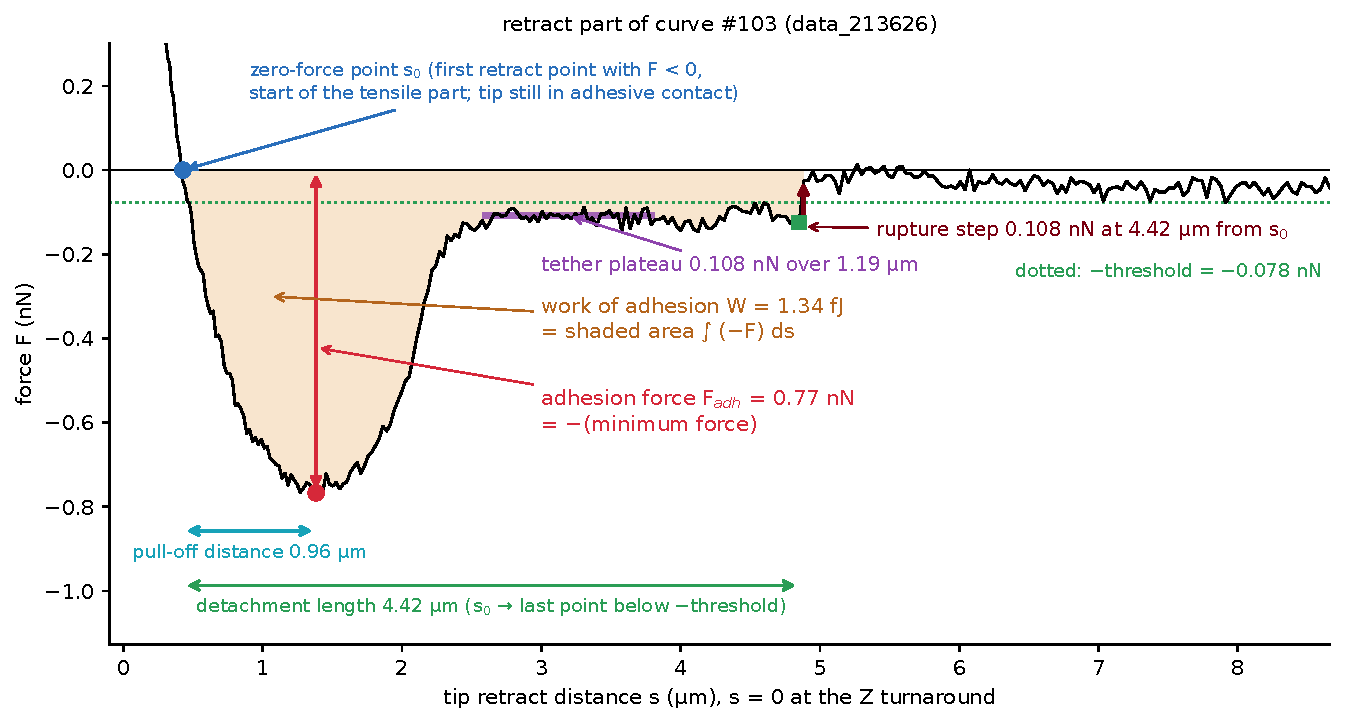
\includegraphics[width=\textwidth]{fig/overview.pdf}
\end{column}
\begin{column}{0.35\textwidth}\scriptsize
\textcolor{cBlue}{$\bullet$ \textbf{$s_0$}} first retract point with $F<0$ \tagM\\[2pt]
\textcolor{cRed}{$\bullet$ \textbf{Adhesion force} $F_\text{adh}$} $=-\min F$ \tagM\\[2pt]
\textcolor{cTeal}{$\bullet$ \textbf{Pull-off distance}} $s_0\to$ minimum \tagM\\[2pt]
\textcolor{cGreen}{$\bullet$ \textbf{Detachment length}} $s_0\to$ last point below $-$threshold \tagC\\[2pt]
\textcolor{cGreen}{$\bullet$ \textbf{Detached flag}} 1 if the force returned to baseline before the end \tagC\\[2pt]
\textcolor{cOrange}{$\bullet$ \textbf{Work of adhesion} $W$} $=\int(-F)\,ds$, shaded area \tagC\\[2pt]
\textcolor{cDRed}{$\bullet$ \textbf{Rupture events}} number, position and height of sudden force jumps \tagD\\[2pt]
\textcolor{cPurple}{$\bullet$ \textbf{Tether plateau}} force and length of a flat attractive segment \tagD\\[2pt]
\textcolor{cRed}{$\bullet$ \textbf{JKR $w$}} $=2F_\text{adh}/(3\pi R)$, not drawn \tagMo\\[6pt]
\tagM~read off the curve\\
\tagC~needs a threshold or an integral\\
\tagD~pattern recognition\\
\tagMo~needs a contact model
\end{column}
\end{columns}
\end{frame}

\begin{frame}{Overview table (values for data\_213626, 2775 curves)}
\scriptsize\renewcommand{\arraystretch}{1.0}
\begin{tabularx}{\textwidth}{@{}p{3.3cm} l X l l@{}}
\toprule
property \quad\texttt{map name} & how & definition (on the retract curve) & unit & median [5--95\,\%]\\
\midrule
adhesion force \newline\texttt{adh\_force\_nN} & \tagM & $-\min F$ after $s_0$ & \si{\nano\newton} & 0.95 [0.28--1.77]\\
pull-off distance \newline\texttt{adh\_pulloff\_um} & \tagM & $s(F_\text{min})-s_0$ & \si{\micro\metre} & 0.94 [0.60--1.97]\\
work of adhesion \newline\texttt{adh\_work\_fJ} & \tagC & $\int_{s_0}^{s_\text{end}}(-F)\,ds$ & \si{\femto\joule} & 1.42 [0.71--2.33]\\
detachment length \newline\texttt{adh\_length\_um} & \tagC & $s_\text{end}-s_0$, $s_\text{end}$ = last point below $-$threshold & \si{\micro\metre} & 3.2 [2.1--8.0]\\
detached \newline\texttt{adh\_detached} & \tagC & 1 if $s_\text{end}$ lies before the end of the retract & 0/1 & 92\,\% detached\\
rupture events \newline\texttt{adh\_n\_ruptures} & \tagD & number of sudden steps towards 0 & -- & 14\,\% of curves $\ge 1$\\
last rupture position \newline\texttt{adh\_last\_rupture\_um} & \tagD & $s(\text{last step})-s_0$ & \si{\micro\metre} & 1.6 [1.0--4.5]$^{*}$\\
last rupture step \newline\texttt{adh\_last\_rupture\_nN} & \tagD & height of the last step & \si{\nano\newton} & 0.10 [0.07--0.21]$^{*}$\\
tether force \newline\texttt{adh\_tether\_nN} & \tagD & $-$median $F$ on the last flat plateau & \si{\nano\newton} & 0.070 [0.043--0.165]$^{\dagger}$\\
tether length \newline\texttt{adh\_tether\_len\_um} & \tagD & length of that plateau & \si{\micro\metre} & 1.08 [0.82--2.24]$^{\dagger}$\\
JKR work of adhesion $w$ \newline\texttt{adh\_gamma\_JKR\_mJ\_m2} & \tagMo & $2F_\text{adh}/(3\pi R)$, $R=\SI{3}{\micro\metre}$ & \si{\milli\joule\per\square\metre} & 0.067 [0.020--0.125]\\
\bottomrule
\end{tabularx}\\[1pt]
\tiny $^{*}$ only the 384 curves with $\ge1$ rupture.\quad $^{\dagger}$ only the 355 curves (12.8\,\%) with a tether plateau; curves without one have 0.
\end{frame}

% ---------------------------------------------------------------------------
\section{Distance axis}

\begin{frame}{Distances are measured along the tip position, not the stage position}
\begin{columns}[T]
\begin{column}{0.40\textwidth}
\centering
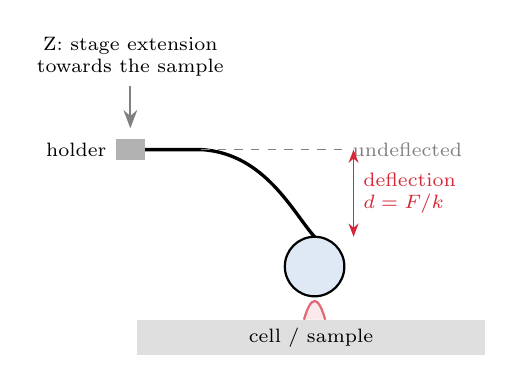
\begin{tikzpicture}[scale=0.9,>=Stealth]
 % sample
 \fill[gray!25] (-0.3,0) rectangle (4.6,-0.5); \node[font=\scriptsize] at (2.15,-0.25) {cell / sample};
 % adhesive neck
 \draw[thick,cRed!70,fill=cRed!10] (2.05,0) .. controls (2.15,0.35) and (2.25,0.35) .. (2.35,0.0);
 % bead
 \draw[thick,fill=cBlue!15] (2.2,0.75) circle (0.42);
 % cantilever bent DOWN (pulled by adhesion)
 \draw[very thick] (-0.2,2.4) -- (0.6,2.4) .. controls (1.5,2.35) and (1.9,1.5) .. (2.2,1.17);
 \draw[dashed,gray] (0.6,2.4) -- (2.6,2.4) node[right,font=\scriptsize]{undeflected};
 % stage / base
 \fill[gray!60] (-0.6,2.25) rectangle (-0.2,2.55); \node[font=\scriptsize,anchor=east] at (-0.6,2.4) {holder};
 % deflection
 \draw[<->,cRed] (2.75,2.4) -- (2.75,1.17) node[midway,right,font=\scriptsize,align=left]{deflection\\$d=F/k$};
 % Z arrow
 \draw[->,thick,gray] (-0.4,3.3) -- (-0.4,2.7); \node[above,font=\scriptsize,align=center] at (-0.4,3.3) {Z: stage extension\\towards the sample};
\end{tikzpicture}
\end{column}
\begin{column}{0.58\textwidth}\small
\begin{itemize}
\item The stage moves by $Z$, but the probe also moves relative to the holder because the cantilever bends: $d=F/k$.
\item \textbf{Tip position} $s_\text{tip}=Z-F/k$ (with $k=\SI{90}{\nano\newton\per\micro\metre}$).
\item \textbf{Retract distance} $s=s_\text{tip}(\text{turnaround})-s_\text{tip}$, so $s=0$ at the turnaround and increases while pulling away.
\item All distances (pull-off, detachment, rupture, tether) are differences of $s$, measured from $s_0$.
\item Size of the correction here: $\SI{1}{\nano\newton}\leftrightarrow\SI{11}{\nano\metre}$. It reaches about \SI{40}{\nano\metre}, i.e. \SI{\approx1}{\percent} of the micrometre distances (next slide). It matters for softer cantilevers or larger forces.
\end{itemize}
\end{column}
\end{columns}
\end{frame}

\begin{frame}{Tip versus stage travel on the example curve}
\centering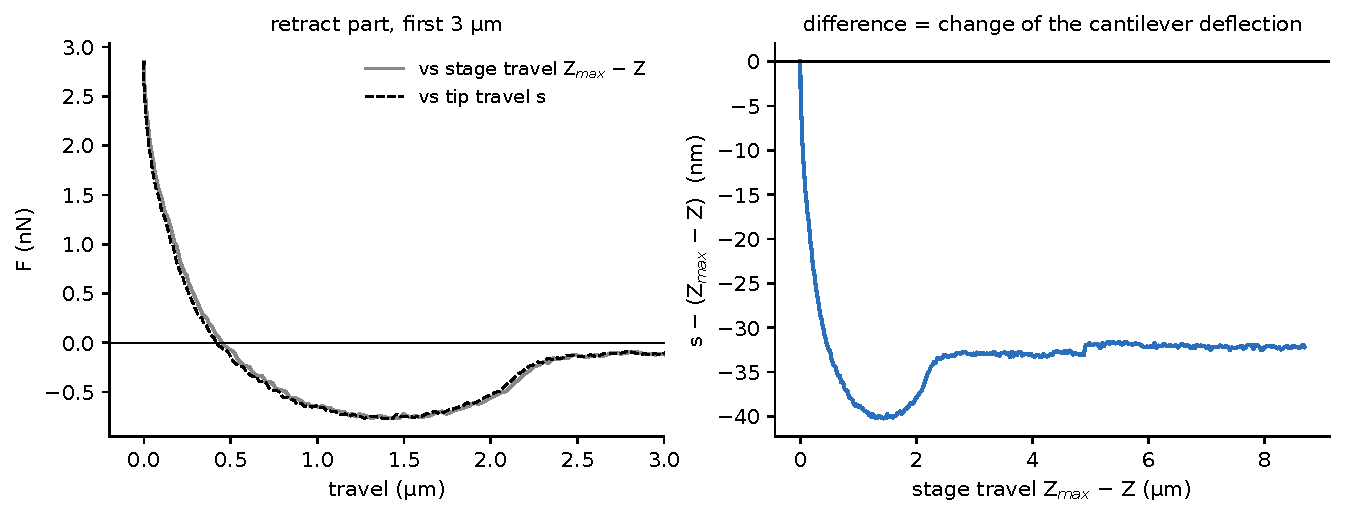
\includegraphics[width=0.95\textwidth]{fig/tip_vs_z.pdf}
\small
\begin{itemize}
\item Left: the curve hardly changes when plotted against tip travel instead of stage travel.
\item Right: the difference equals the change of the cantilever deflection, from the peak load (\SI{2.9}{\nano\newton} $\to$ \SI{32}{\nano\metre}) to the adhesion minimum ($-$\SI{0.77}{\nano\newton} $\to -$\SI{8.5}{\nano\metre}): about \SI{40}{\nano\metre} in total.
\end{itemize}
\end{frame}

% ---------------------------------------------------------------------------
\section{Read directly from the curve}

\begin{frame}{Zero-force point $s_0$ and adhesion force $F_\text{adh}$ \tagM}
\begin{columns}[T]
\begin{column}{0.5\textwidth}\small
\textbf{Zero-force point $s_0$}
\begin{itemize}
\item The first retract point with $F<0$.
\item From here on the sample pulls on the probe (tensile contact).
\item \textbf{The probe is still in contact at $s_0$.} With adhesion, contact persists under tension. $s_0$ is the reference point for all distances, not the moment of separation.
\end{itemize}
\textbf{Adhesion force}
\[F_\text{adh}=-\min_{s\ge s_0}F(s)\]
\begin{itemize}
\item The largest tensile force the contact sustains (``pull-off force'').
\item Raw data, single point, no fit and no smoothing.
\end{itemize}
\end{column}
\begin{column}{0.48\textwidth}\small
\textbf{What it reflects}
\begin{itemize}
\item the number and strength of bonds and contacts formed during the dwell, and the contact area
\item depends on the loading history: trigger force, contact time, retract speed (bonds are rate dependent)
\end{itemize}
\textbf{Precision}
\begin{itemize}
\item noise per point $\sigma\approx\SI{12}{\pico\newton}$
\item the minimum of noisy data is biased towards more negative values by about $1$--$3\,\sigma$ ($\lesssim\SI{0.04}{\nano\newton}$). This is small against typical $F_\text{adh}\approx\SI{1}{\nano\newton}$.
\end{itemize}
\textbf{Example (curve \#103)}: $F_\text{adh}=\SI{0.77}{\nano\newton}$
\end{column}
\end{columns}
\end{frame}

\begin{frame}{Pull-off distance \tagM}
\begin{columns}[T]
\begin{column}{0.48\textwidth}
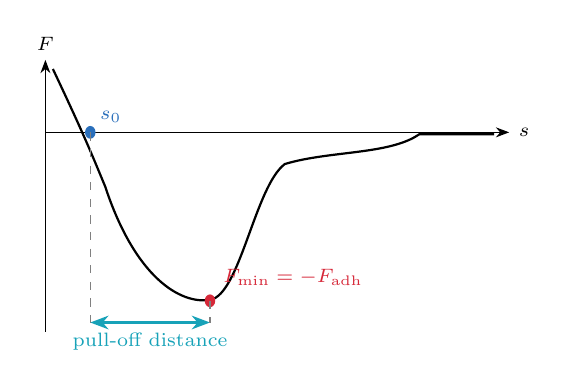
\begin{tikzpicture}[xscale=0.95,yscale=1.15,>=Stealth]
 \draw[->] (0,0) -- (6.2,0) node[right,font=\scriptsize]{$s$};
 \draw[->] (0,-2.2) -- (0,0.8) node[above,font=\scriptsize]{$F$};
 \draw[thick] (0.1,0.7) .. controls (0.5,0) and (0.6,-0.2) .. (0.8,-0.6) .. controls (1.2,-1.6) and (1.8,-1.9) .. (2.2,-1.85)
   .. controls (2.6,-1.8) and (2.8,-0.6) .. (3.2,-0.35) .. controls (3.8,-0.2) and (4.6,-0.25) .. (5.0,-0.02) -- (6,-0.02);
 \fill[cBlue] (0.6,0) circle (2pt) node[above right,font=\scriptsize,cBlue]{$s_0$};
 \fill[cRed] (2.2,-1.86) circle (2pt);
 \draw[<->,cTeal,thick] (0.6,-2.1) -- (2.2,-2.1) node[midway,below,font=\scriptsize]{pull-off distance};
 \draw[dashed,gray] (0.6,0) -- (0.6,-2.1); \draw[dashed,gray] (2.2,-1.86) -- (2.2,-2.1);
 \node[font=\scriptsize,cRed,right] at (2.25,-1.6) {$F_\text{min}=-F_\text{adh}$};
\end{tikzpicture}
\end{column}
\begin{column}{0.5\textwidth}\small
\[d_\text{pull-off}=s(F_\text{min})-s_0\]
\begin{itemize}
\item How far the probe is pulled, starting where the force turns tensile, until the tensile force is largest.
\item On a cell this includes stretching of the membrane, the cortex and the bonds before they start to give way.
\item Read from the position of the same raw minimum as $F_\text{adh}$.
\item Typical: \SI{0.94}{\micro\metre} [0.60--1.97]; curve \#103: \SI{0.96}{\micro\metre}.
\item The minimum is broad on cells. Because of noise its position can shift by a few points (\num{\approx 0.1}\,\si{\micro\metre}).
\end{itemize}
\end{column}
\end{columns}
\end{frame}

% ---------------------------------------------------------------------------
\section{Threshold-based quantities}

\begin{frame}{The noise threshold (decides ``still attached'' and the minimum step size) \tagC}
\centering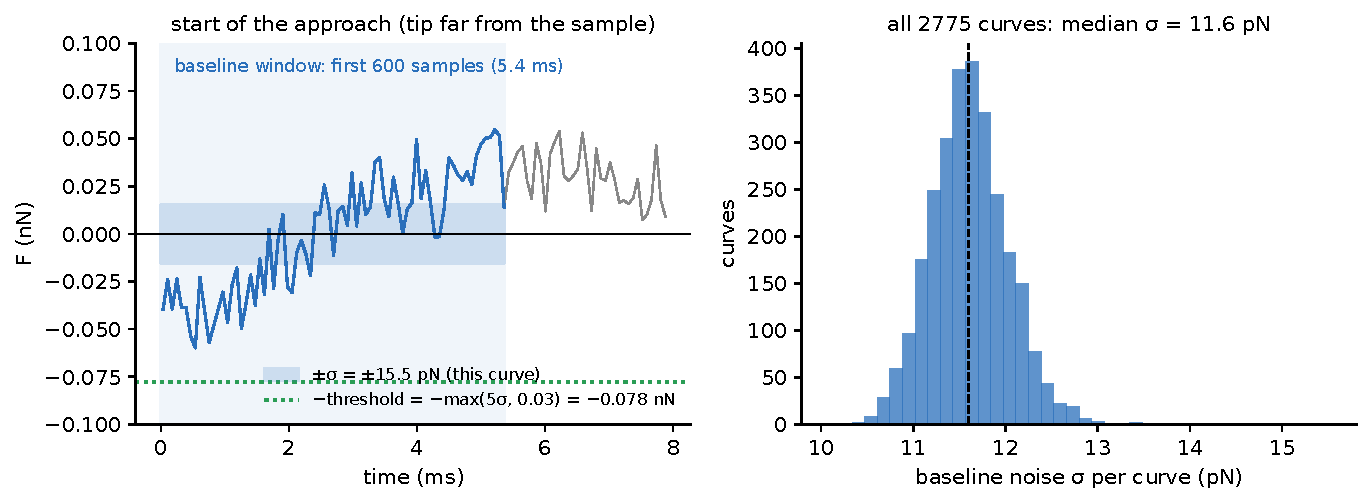
\includegraphics[width=0.92\textwidth]{fig/noise.pdf}
\small
\begin{itemize}
\item $\sigma$ = standard deviation of the force in the baseline window (the first 600 raw samples, \SI{5.4}{\milli\second}, after drag correction), divided by $\sqrt8$ for the block averaging.
\item \textbf{threshold} $=\max(5\sigma,\ \SI{0.03}{\nano\newton})$. Median over all curves: $\sigma=\SI{11.6}{\pico\newton}$, threshold $=\SI{0.058}{\nano\newton}$.
\item Any slow drift inside the baseline window is included in $\sigma$, so the threshold errs on the conservative side (curve \#103: \SI{0.078}{\nano\newton}).
\end{itemize}
\end{frame}

\begin{frame}{Detachment length and the ``detached'' flag \tagC}
\centering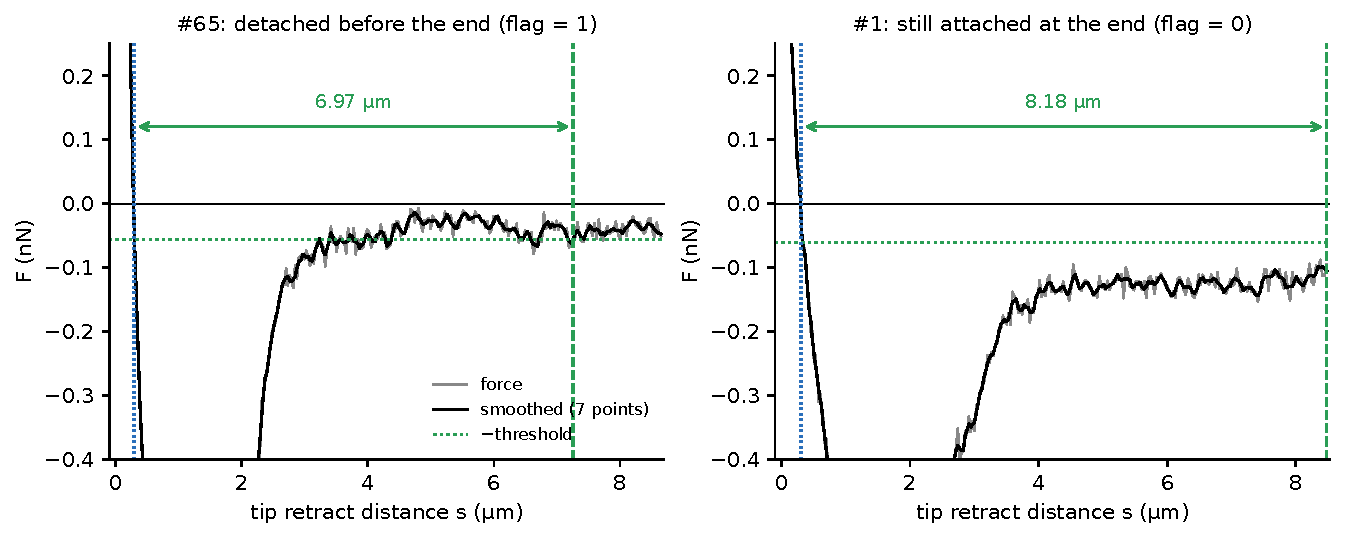
\includegraphics[height=0.37\textheight]{fig/detachment.pdf}
\begin{columns}[T]
\begin{column}{0.5\textwidth}\small
\begin{enumerate}
\item Smooth the retract force: Savitzky--Golay filter, 7 points ($\approx\SI{0.24}{\micro\metre}$), 2nd order.
\item $s_\text{end}$ = the \textbf{last} point after $s_0$ where the smoothed force is $<-$threshold.
\item \textbf{Detachment length} $L=s_\text{end}-s_0$.
\end{enumerate}
\end{column}
\begin{column}{0.48\textwidth}\small
\begin{itemize}
\item \textbf{detached} = 1 if $s_\text{end}$ lies at least 6 points ($\approx\SI{0.2}{\micro\metre}$) before the end of the retract; otherwise 0.
\item detached = 0: still attached when the retract stopped ($\approx\SI{8.7}{\micro\metre}$), so $L$, $W$ and the tether length are \textbf{lower bounds}. This applies to 8\,\% of the curves.
\item Slow tails close to the threshold make $L$ sensitive: left, $L=\SI{6.97}{\micro\metre}$ although most of the force is gone by $\approx\SI{3}{\micro\metre}$.
\end{itemize}
\end{column}
\end{columns}
\end{frame}

\begin{frame}{Work of adhesion $W$ \tagC}
\begin{columns}[T]
\begin{column}{0.55\textwidth}
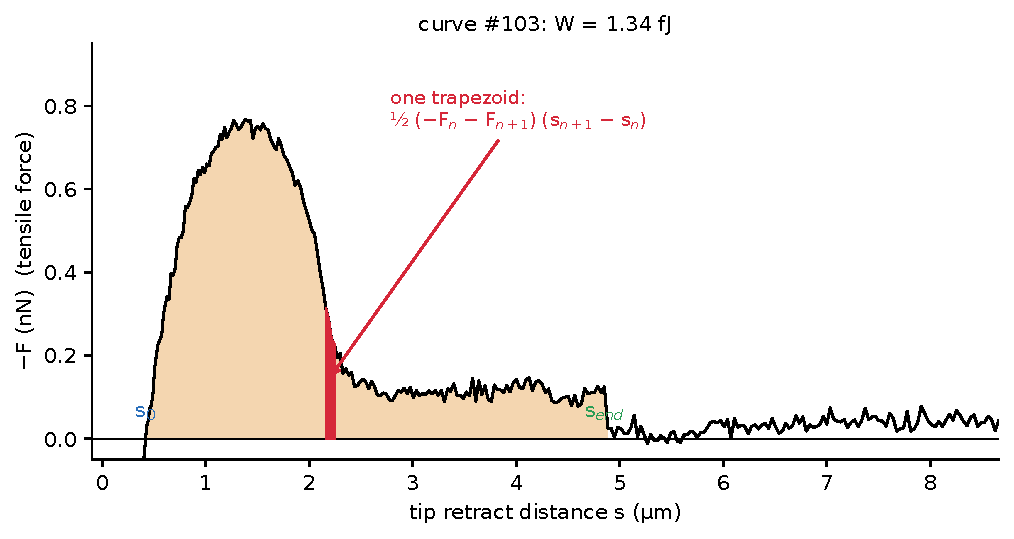
\includegraphics[width=\textwidth]{fig/work.pdf}
\end{column}
\begin{column}{0.44\textwidth}\small
\[W=\int_{s_0}^{s_\text{end}}\max\bigl(-F(s),0\bigr)\,ds\]
\begin{itemize}
\item The mechanical work needed to separate the probe from the sample: the area between the tensile part of the curve and $F=0$.
\item Computed with the trapezoid rule on the raw points from $s_0$ to one point past $s_\text{end}$. Positive excursions (noise) count as 0.
\item Unit: $\si{\nano\newton}\cdot\si{\micro\metre}=\SI{1}{\femto\joule}=\SI{e-15}{\joule}$.
\item Collects everything: bond unbinding, deformation of the cell surface, tethers.
\item Curve \#103: $W=\SI{1.34}{\femto\joule}$; typical \SI{1.42}{\femto\joule} [0.71--2.33].
\item A lower bound if not detached. Not normalised by contact area.
\end{itemize}
\end{column}
\end{columns}
\end{frame}

% ---------------------------------------------------------------------------
\section{Rupture events}

\begin{frame}{Rupture events: what they are}
\begin{columns}[T]
\begin{column}{0.46\textwidth}
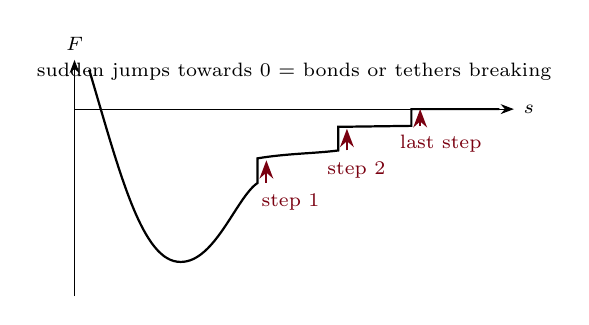
\begin{tikzpicture}[xscale=0.93,yscale=1.25,>=Stealth]
 \draw[->] (0,0) -- (6,0) node[right,font=\scriptsize]{$s$};
 \draw[->] (0,-1.9) -- (0,0.5) node[above,font=\scriptsize]{$F$};
 \draw[thick] (0.2,0.4) .. controls (0.6,-0.6) and (0.9,-1.5) .. (1.4,-1.55) .. controls (1.9,-1.6) and (2.2,-0.9) .. (2.5,-0.75)
     -- (2.5,-0.5) .. controls (2.9,-0.45) and (3.3,-0.45) .. (3.6,-0.42) -- (3.6,-0.18) -- (4.6,-0.17) -- (4.6,0) -- (5.8,0);
 \draw[->,cDRed,thick] (2.62,-0.75) -- (2.62,-0.52); \node[font=\scriptsize,cDRed] at (2.95,-0.95) {step 1};
 \draw[->,cDRed,thick] (3.72,-0.42) -- (3.72,-0.2); \node[font=\scriptsize,cDRed] at (3.85,-0.62) {step 2};
 \draw[->,cDRed,thick] (4.72,-0.17) -- (4.72,0.0); \node[font=\scriptsize,cDRed] at (5.0,-0.35) {last step};
 \node[font=\scriptsize,align=center] at (3,0.38) {sudden jumps towards 0 = bonds or tethers breaking};
\end{tikzpicture}
\end{column}
\begin{column}{0.52\textwidth}\small
\begin{itemize}
\item While the probe is pulled away it is held by bonds (receptor--ligand, membrane anchors) and possibly by membrane tethers.
\item When one of them breaks, its share of the force is lost at once and the force \textbf{jumps towards 0 from one point to the next}.
\item Smooth unbinding (many small contacts letting go gradually) gives a steep but \textbf{continuous} rise. That is \textbf{not} counted.
\item Outputs:
 \begin{itemize}
 \item \texttt{adh\_n\_ruptures}: number of steps after the force minimum
 \item \texttt{adh\_last\_rupture\_um}: position of the last step (from $s_0$)
 \item \texttt{adh\_last\_rupture\_nN}: height of the last step, i.e. the force carried by the last bond or tether
 \end{itemize}
\end{itemize}
\end{column}
\end{columns}
\end{frame}

\begin{frame}{Rupture events: how a step is detected \tagD}
\centering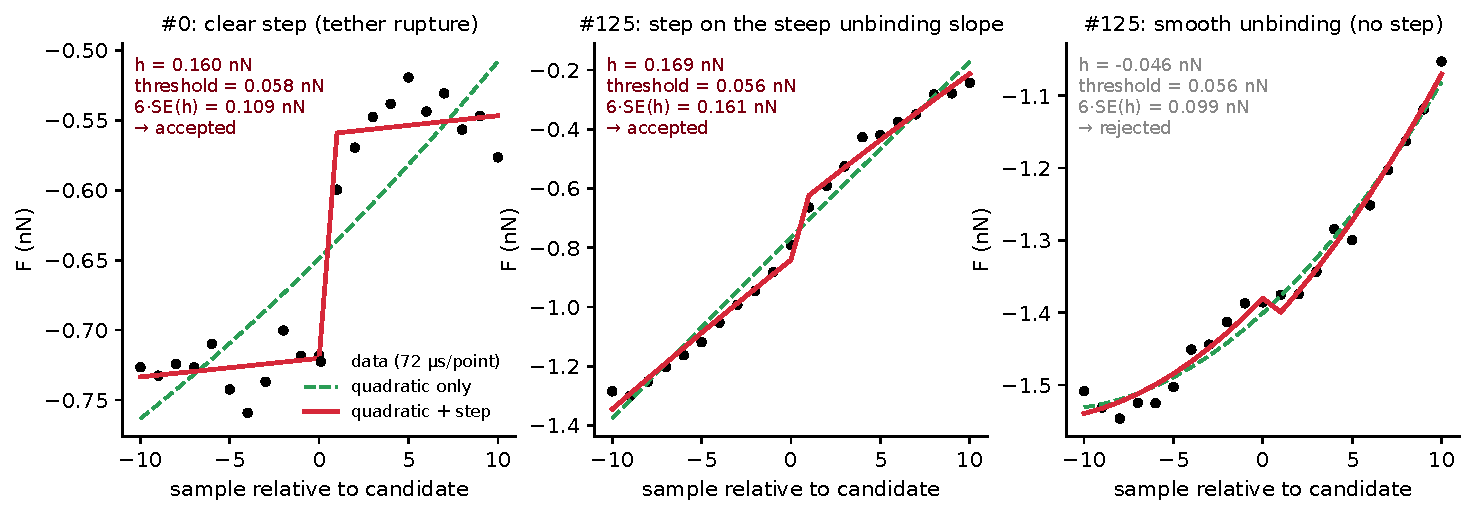
\includegraphics[height=0.42\textheight]{fig/rupture_fit.pdf}\\[-2pt]
\begin{columns}[T]
\begin{column}{0.53\textwidth}\scriptsize
For every point $i$ between the force minimum and $s_\text{end}$ (+6 points):
\begin{enumerate}
\item pre-filter: mean of the next 3 points $-$ mean of the last 3 points $\ge$ threshold/2
\item least-squares fit in a window of $\pm10$ points ($\approx\pm\SI{0.34}{\micro\metre}$):\\
 $F(x)=a+b\,x+c\,x^2+h\cdot[x>0]$ ($x$ = point index $-\,i$)\\
 the quadratic absorbs any smooth trend, $h$ is the step
\end{enumerate}
\end{column}
\begin{column}{0.45\textwidth}\scriptsize
Accept the step if all hold:
\begin{itemize}
\item $h\ \ge$ threshold ($\approx\SI{0.058}{\nano\newton}$)
\item $h\ \ge 6\,\mathrm{SE}(h)$, with $\mathrm{SE}(h)=\sigma_\text{eff}\sqrt{[(X^\top X)^{-1}]_{hh}}$ and $\sigma_\text{eff}=\max(\text{fit residual SD},\,\sigma)$
\item still attached just before: smoothed $F$ three points earlier $<-$threshold
\end{itemize}
Steps closer than 10 points are merged (the larger $h$ is kept).
\end{column}
\end{columns}
\end{frame}

\begin{frame}{Rupture events: reading the results}
\small
\begin{itemize}
\item Panel 1 (\#0): a clean step on a flat segment, $h=\SI{0.160}{\nano\newton}$, more than 6\,SE ($=\SI{0.109}{\nano\newton}$), accepted. Typical for a tether letting go.
\item Panel 2 (\#125): a one-point jump on top of the steep unbinding slope, $h=\SI{0.169}{\nano\newton}>6\,\mathrm{SE}=\SI{0.161}{\nano\newton}$, accepted. Steps on slopes need to be larger because the fit is less certain there.
\item Panel 3 (same curve, 14 points earlier): steep but continuous, $h\approx 0$ (the quadratic alone describes it), rejected.
\end{itemize}
\textbf{In data\_213626}: 86\,\% of curves have no rupture, 13\,\% have one, 1\,\% have two or more. Last step: \SI{0.10}{\nano\newton} [0.07--0.21], at \SI{1.6}{\micro\metre} [1.0--4.5] from $s_0$.\\[6pt]
\textbf{Limits}
\begin{itemize}
\item steps smaller than the threshold ($\approx\SI{0.06}{\nano\newton}$) are not detected
\item two ruptures within 10 points ($\approx\SI{0.34}{\micro\metre}$) count as one
\item time resolution \SI{72}{\micro\second} per point: a ``step'' is any change between two consecutive points
\item if there is no rupture, position and height are empty (NaN)
\end{itemize}
\end{frame}

% ---------------------------------------------------------------------------
\section{Membrane tethers}

\begin{frame}{Membrane tethers: what a force plateau means}
\begin{columns}[T]
\begin{column}{0.45\textwidth}
\centering
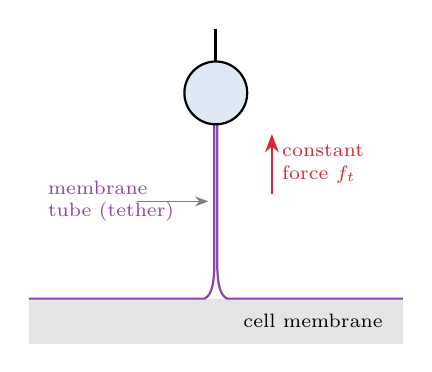
\begin{tikzpicture}[scale=0.95,>=Stealth]
 \fill[gray!20] (-0.5,0) rectangle (4.5,-0.6);
 \draw[thick,cPurple] (-0.5,0) -- (1.85,0) .. controls (1.95,0.05) and (1.97,0.2) .. (1.98,0.4) -- (1.98,2.35);
 \draw[thick,cPurple] (4.5,0) -- (2.15,0) .. controls (2.05,0.05) and (2.03,0.2) .. (2.02,0.4) -- (2.02,2.35);
 \node[font=\scriptsize] at (3.3,-0.3) {cell membrane};
 \draw[thick,fill=cBlue!15] (2,2.75) circle (0.42);
 \draw[very thick] (2,3.17) -- (2,3.6);
 \draw[->,thick,cRed] (2.75,1.4) -- (2.75,2.2) node[midway,right,font=\scriptsize,align=left]{constant\\force $f_t$};
 \node[font=\scriptsize,cPurple,align=left] at (0.6,1.3) {membrane\\tube (tether)};
 \draw[->,gray] (0.95,1.3) -- (1.9,1.3);
\end{tikzpicture}
\end{column}
\begin{column}{0.53\textwidth}\small
\begin{itemize}
\item If the probe stays bound to the membrane after the bulk contact has let go, a thin \textbf{membrane tube} (tether) is pulled out of the cell.
\item A tether gets longer at a nearly \textbf{constant force}, so the retract curve shows a \textbf{flat plateau} at $F<0$.
\item The plateau ends when the anchor breaks (a rupture step to 0), or continues past the end of the retract.
\item Several tethers in parallel give one plateau at the summed force (and steps between levels).
\item Background, not computed here: for a static tether $f_t=2\pi\sqrt{2\kappa\,\sigma_m}$ (bending rigidity $\kappa$, membrane tension $\sigma_m$). At a finite pulling speed $f_t$ is higher (viscous contribution).
\end{itemize}
\end{column}
\end{columns}
\end{frame}

\begin{frame}{Tether plateaus: how they are detected \tagD}
\centering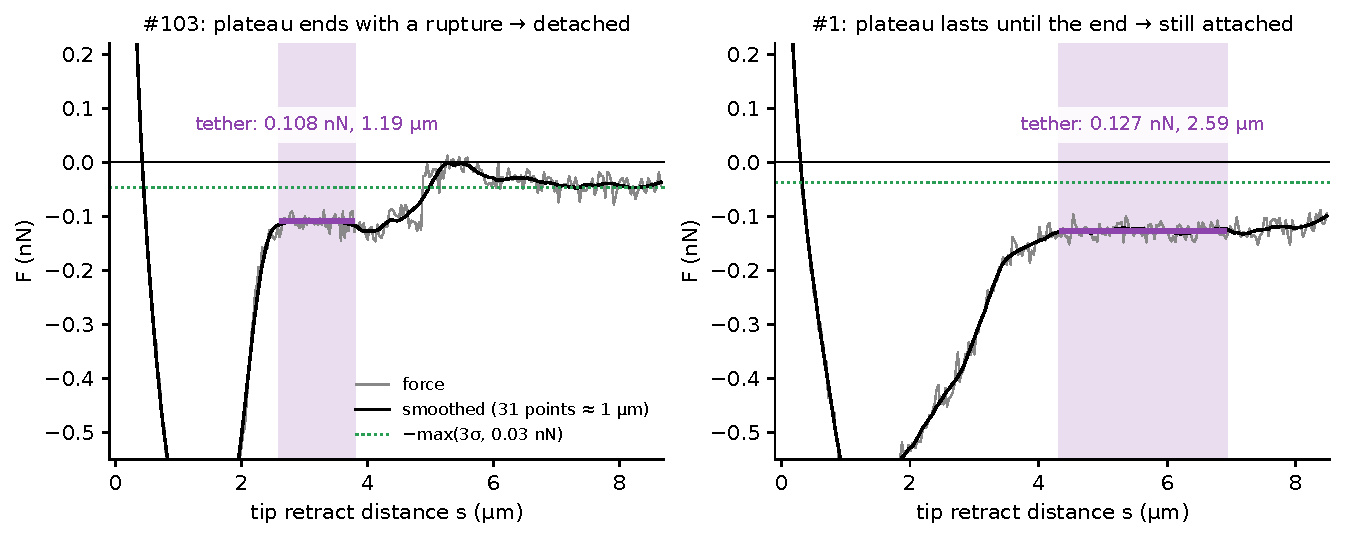
\includegraphics[height=0.40\textheight]{fig/tether.pdf}
\begin{columns}[T]
\begin{column}{0.52\textwidth}\scriptsize
\begin{enumerate}
\item Smooth the retract force strongly: Savitzky--Golay, 31 points ($\approx\SI{2.2}{\milli\second}\approx\SI{1}{\micro\metre}$), 2nd order.
\item Between the force minimum and $s_\text{end}$, mark points with
 smoothed $F<-\max(3\sigma,\SI{0.03}{\nano\newton})$ (still attractive) and
 $|dF/ds|<\SI{0.05}{\nano\newton\per\micro\metre}$ (flat).
\item Keep runs of marked points at least \SI{0.8}{\micro\metre} long; take the \textbf{last} run (closest to detachment).
\end{enumerate}
\end{column}
\begin{column}{0.46\textwidth}\scriptsize
\begin{itemize}
\item \textbf{tether force} = $-$median of the raw force on that run
\item \textbf{tether length} = length of the run (\si{\micro\metre})
\item no run: both 0
\item Left: \SI{0.108}{\nano\newton} over \SI{1.19}{\micro\metre}, ends with a \SI{0.108}{\nano\newton} rupture step (the same force, as expected when a single tether lets go).
\item Right: \SI{0.127}{\nano\newton} over $\ge\SI{2.59}{\micro\metre}$, still attached: the length is a lower bound.
\item In data\_213626: 12.8\,\% of curves, \SI{0.070}{\nano\newton} [0.043--0.165], \SI{1.08}{\micro\metre} [0.82--2.24].
\end{itemize}
\end{column}
\end{columns}
\end{frame}

% ---------------------------------------------------------------------------
\section{Contact model}

\begin{frame}{JKR work of adhesion per area $w$ \tagMo}
\begin{columns}[T]
\begin{column}{0.42\textwidth}
\centering
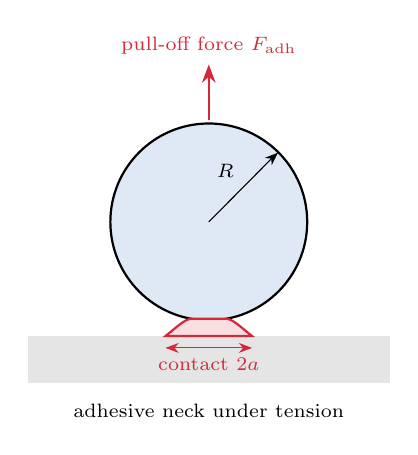
\begin{tikzpicture}[scale=1.0,>=Stealth]
 \fill[gray!20] (-0.3,0) rectangle (4.3,-0.6);
 \draw[thick,fill=cBlue!15] (2,1.45) circle (1.25);
 \draw[thick,cRed,fill=cRed!15] (1.45,0) .. controls (1.6,0.12) and (1.7,0.22) .. (1.78,0.22) -- (2.22,0.22) .. controls (2.3,0.22) and (2.4,0.12) .. (2.55,0) -- cycle;
 \draw[<->,cRed] (1.45,-0.15) -- (2.55,-0.15) node[midway,below,font=\scriptsize]{contact $2a$};
 \draw[->] (2,1.45) -- (2.88,2.33) node[midway,above left,font=\scriptsize]{$R$};
 \draw[->,thick,cRed] (2,2.75) -- (2,3.45) node[above,font=\scriptsize]{pull-off force $F_\text{adh}$};
 \node[font=\scriptsize,align=center] at (2,-0.95) {adhesive neck under tension};
\end{tikzpicture}
\end{column}
\begin{column}{0.56\textwidth}\small
\textbf{Model}: elastic sphere (radius $R$) on an elastic flat with surface adhesion; JKR theory (Johnson--Kendall--Roberts, 1971). The pull-off force is
\[F_\text{adh}=\tfrac32\,\pi R\,w\quad\Longrightarrow\quad w=\frac{2F_\text{adh}}{3\pi R}\]
$w$: work of adhesion per unit area (Dupré), the energy needed to separate a unit area of contact.
\begin{itemize}
\item $R=\SI{3}{\micro\metre}$ (estimated from topography, not measured)
\item units: $\si{\nano\newton\per\micro\metre}=\si{\milli\joule\per\square\metre}$
\item example: $w=\dfrac{2\cdot\SI{0.952}{\nano\newton}}{3\pi\cdot\SI{3}{\micro\metre}}=\SI{0.067}{\milli\joule\per\square\metre}$ (median)
\item stiff, weakly adhesive contacts (DMT limit): $F_\text{adh}=2\pi Rw$, giving a $w$ that is $\times0.75$ smaller
\end{itemize}
\end{column}
\end{columns}
\end{frame}

\begin{frame}{JKR $w$: how to use it}
\small
\begin{itemize}
\item $w$ is $F_\text{adh}$ multiplied by a constant ($2/(3\pi R)$): the map has \textbf{exactly the same pattern} as the adhesion force map. It only converts force to energy per area.
\item JKR assumes an elastic contact, uniform surface energy, quasi-static separation and full contact until pull-off. Living cells are viscoelastic and adhere through discrete bonds and tethers, so these assumptions are not met.
\item Use $w$ as an \textbf{apparent, comparative} quantity (same probe, same loading), or to compare with literature values given per area. Do not read it as a true surface energy.
\item $R$ enters as $1/R$: an error in $R$ rescales every $w$ by the same factor.
\item For a model-free measure of the total separation energy, use the work of adhesion $W$ (\si{\femto\joule}). It includes everything (bonds, tethers, deformation) but has no area normalisation.
\end{itemize}
\end{frame}

% ---------------------------------------------------------------------------
\section{Results and reference}

\begin{frame}{Example maps (data\_213626, 37.5 $\times$ 37.5 \si{\micro\metre})}
\begin{columns}[T]
\begin{column}{0.58\textwidth}
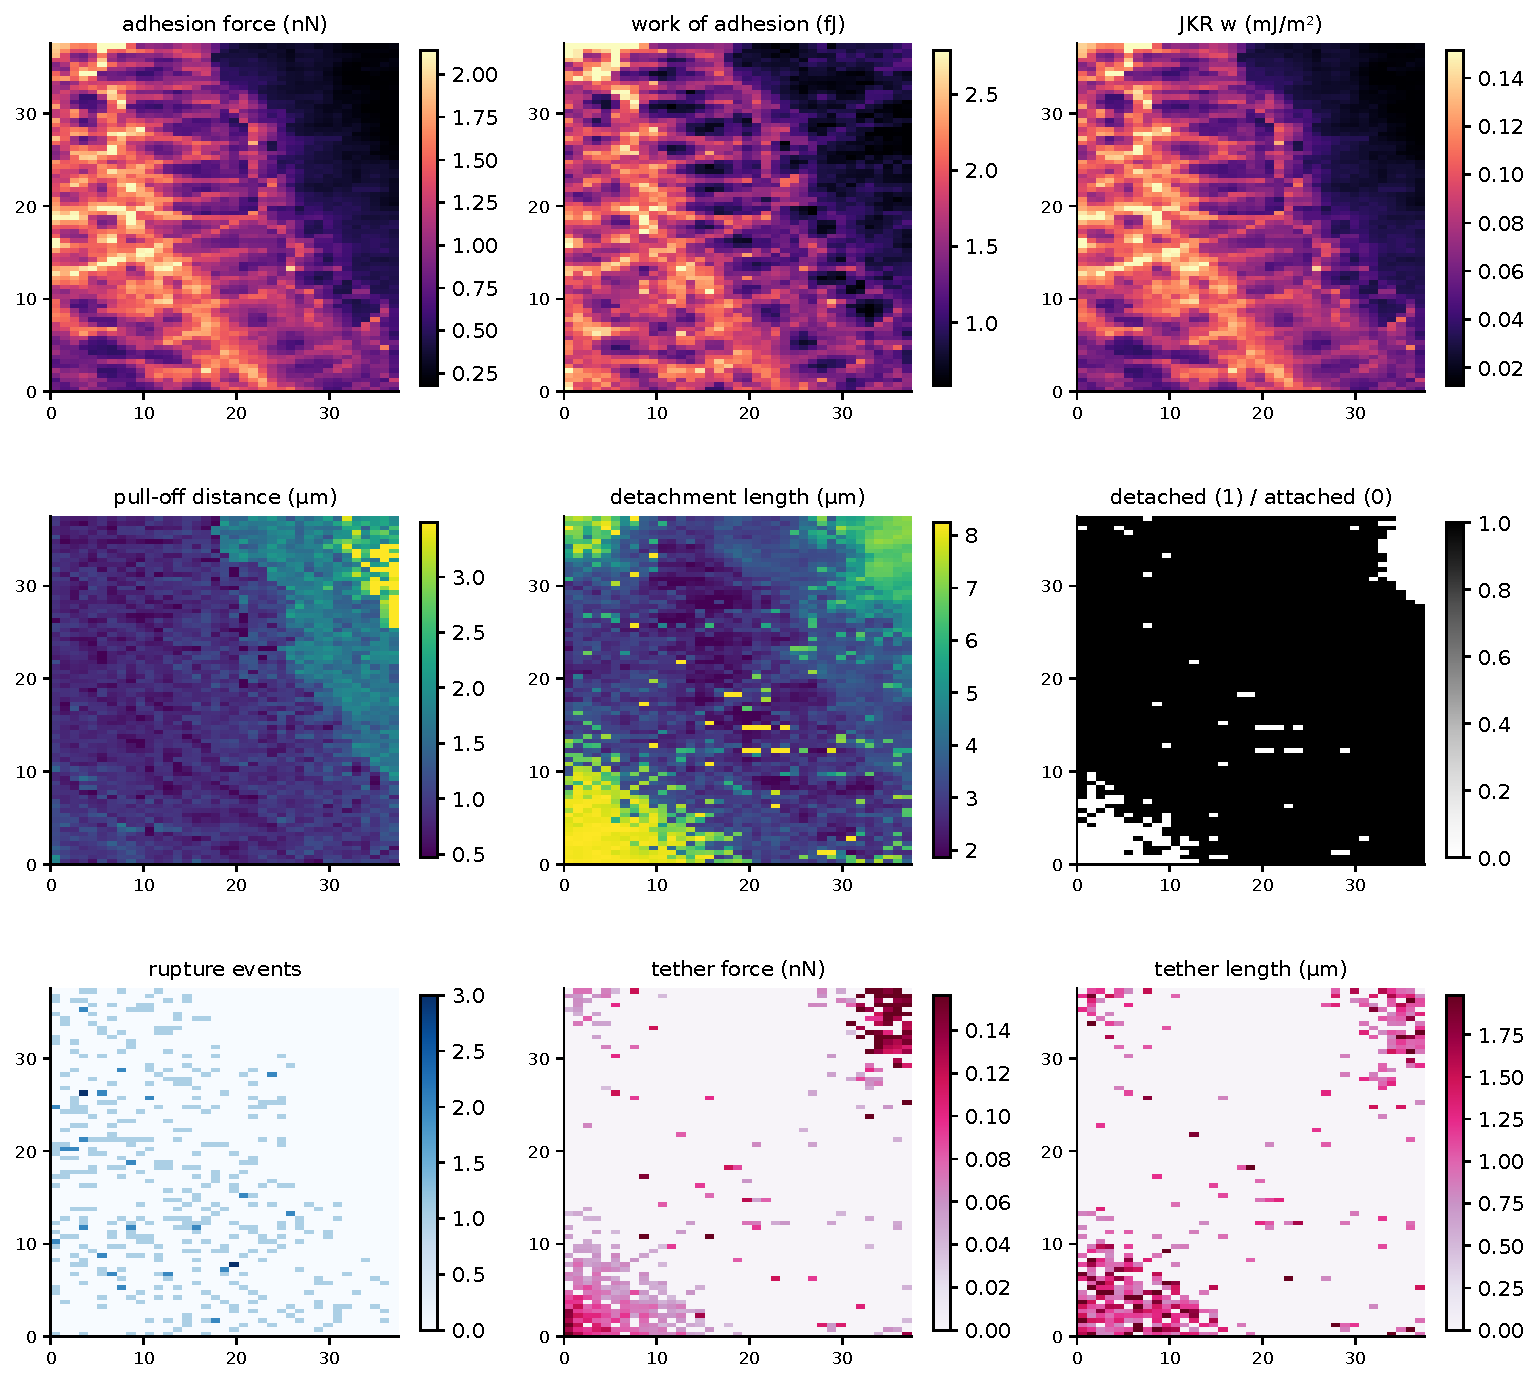
\includegraphics[height=0.82\textheight]{fig/maps.pdf}
\end{column}
\begin{column}{0.40\textwidth}\small
\begin{itemize}
\item Adhesion force and work: high along the left and diagonal band, low in the top-right region.
\item JKR $w$: the adhesion force map scaled by a constant, so the same pattern.
\item Pull-off distance is longer in the right half. Long detachment lengths, tethers and ``still attached'' curves cluster at the top right and bottom left.
\item Ruptures are scattered over the left half and almost absent at the top right; 14\,\% of the curves have one.
\end{itemize}
\end{column}
\end{columns}
\end{frame}

\begin{frame}{All parameters (as implemented)}
\scriptsize
\begin{tabularx}{\textwidth}{@{}l l X@{}}
\toprule
step & value & meaning\\
\midrule
retract part & after $\arg\max Z$ & Z turnaround of the smoothed stage signal\\
force zero & median of first 600 samples & approach baseline, after drag correction\\
noise $\sigma$ & SD(first 600 samples)$/\sqrt8$ & per curve, for block-averaged points\\
threshold & $\max(5\sigma,\SI{0.03}{\nano\newton})$ & ``still attached'' level and minimum step height\\
tip position & $s_\text{tip}=Z-F/k$ & $k=\SI{0.09}{\newton\per\metre}$\\
$s_0$ & first retract point with $F<0$ & reference for all distances\\
$F_\text{adh}$, pull-off & raw minimum after $s_0$ & no smoothing\\
smoothing (detachment) & Savitzky--Golay 7 points, order 2 & $\approx\SI{0.24}{\micro\metre}$\\
detached & $s_\text{end}$ $\ge 6$ points before the end & otherwise 0 (lower bounds)\\
work & trapezoid on raw points, $s_0\to s_\text{end}$ + 1 point & negative contributions set to 0\\
rupture window & $\pm10$ points, quadratic + step & accept: $h\ge$ threshold, $h\ge6\,$SE, attached before; merge $<10$ points\\
tether smoothing & Savitzky--Golay 31 points, order 2 & $\approx\SI{1}{\micro\metre}$\\
tether criteria & $F<-\max(3\sigma,\SI{0.03}{\nano\newton})$, $|dF/ds|<\SI{0.05}{\nano\newton\per\micro\metre}$, $\ge\SI{0.8}{\micro\metre}$ & last run; force = $-$median raw $F$\\
JKR & $w=2F_\text{adh}/(3\pi R)$, $R=\SI{3}{\micro\metre}$ & sphere geometry only\\
\bottomrule
\end{tabularx}\\[4pt]
Implementation: \texttt{adhesion\_curve()} in \texttt{afm\_ting\_pipeline.py} / \texttt{extract\_topo\_E.py}. All values are set in \texttt{[adhesion]} of \texttt{afm\_pipeline.toml}; \texttt{extract\_topo\_E.py --recompute-adhesion} applies new values to the stored curves without refitting.
\end{frame}

\begin{frame}{Limitations and how to read the maps}
\small
\begin{itemize}
\item \textbf{Calibration}: forces, $W$ and $w$ scale with $k\cdot$InvOLS ($k$ is nominal). Distances do not.
\item \textbf{Vertical force}: no correction for surface slope (adhesion is pulled along the probe axis, not the surface normal). On steep flanks a lateral component is not captured.
\item \textbf{Loading history}: $F_\text{adh}$, $W$ and ruptures depend on trigger force, contact time and retract speed (here $\approx\SI{470}{\micro\metre\per\second}$). Compare maps only at the same settings.
\item \textbf{Finite retract range} ($\approx\SI{8.7}{\micro\metre}$): for the 8\,\% of curves still attached at the end, $L$, $W$ and the tether length are lower bounds. Use the detached flag to filter.
\item \textbf{Threshold sensitivity}: slowly decaying tails near $-$threshold make $L$ (and slightly $W$) sensitive. $F_\text{adh}$ and the pull-off distance are not affected.
\item \textbf{Detection limits}: steps $<\SI{0.06}{\nano\newton}$ or closer than $\SI{0.34}{\micro\metre}$ are missed or merged. Plateaus shorter than \SI{0.8}{\micro\metre} or drifting faster than \SI{0.05}{\nano\newton\per\micro\metre} are not counted as tethers.
\item \textbf{No area normalisation} except the JKR model value $w$, which rests on assumptions that cells do not meet.
\end{itemize}
\end{frame}

\begin{frame}{Summary}
\begin{itemize}
\item \tagM~\textbf{Adhesion force} and \textbf{pull-off distance}: read directly from the minimum of the retract curve, relative to the zero-force point $s_0$.
\item \tagC~\textbf{Detachment length}, \textbf{detached flag} and \textbf{work of adhesion}: need a noise threshold ($\max(5\sigma,\SI{0.03}{\nano\newton})$) and an integral along the tip position.
\item \tagD~\textbf{Rupture events}: sudden steps found with a local ``quadratic + step'' fit, so smooth unbinding is not counted.
\item \tagD~\textbf{Tether plateaus}: long, flat, attractive segments (membrane tubes).
\item \tagMo~\textbf{JKR $w$}: the adhesion force converted to energy per area with an elastic contact model. Apparent and comparative only.
\item Every value is computed per force curve, so each property is a map, and all maps are available in the time-lapse viewer.
\end{itemize}
\end{frame}

\end{document}
